\documentclass{article}
\usepackage{graphicx}
\usepackage{booktabs}
\usepackage{tabularx}
\usepackage{hyperref}
\usepackage{pdflscape}
\usepackage{caption}

\captionsetup[figure]{font=footnotesize} % For figure captions

\hypersetup{
    colorlinks=true,       % false: boxed links; true: colored links
    linkcolor=red,          % color of internal links (change box color with linkbordercolor)
    citecolor=green,        % color of links to bibliography
    filecolor=magenta,      % color of file links
    urlcolor=cyan           % color of external links
}

\title{Hazard Analysis\\\progname}

\author{\authname}

\date{}

%% Comments

\usepackage{color}

\newif\ifcomments\commentstrue %displays comments
%\newif\ifcomments\commentsfalse %so that comments do not display

\ifcomments
\newcommand{\authornote}[3]{\textcolor{#1}{[#3 ---#2]}}
\newcommand{\todo}[1]{\textcolor{red}{[TODO: #1]}}
\else
\newcommand{\authornote}[3]{}
\newcommand{\todo}[1]{}
\fi

\newcommand{\wss}[1]{\authornote{blue}{SS}{#1}} 
\newcommand{\plt}[1]{\authornote{magenta}{TPLT}{#1}} %For explanation of the template
\newcommand{\an}[1]{\authornote{cyan}{Author}{#1}}

%% Common Parts

\newcommand{\progname}{Software Engineering} % PUT YOUR PROGRAM NAME HERE
\newcommand{\authname}{Team 2, SyntaxSentinals
\\ Lucas Chen
\\ Dennis Fong
\\ Mohammad Mohsin Khan
\\ Julian Cecchini
\\ Luigi Quattrociocchi} % AUTHOR NAMES                  

\usepackage{hyperref}
    \hypersetup{colorlinks=true, linkcolor=blue, citecolor=blue, filecolor=blue,
                urlcolor=blue, unicode=false}
    \urlstyle{same}
                                


\begin{document}

\maketitle
\thispagestyle{empty}

~\newpage

\pagenumbering{roman}

\begin{table}[hp]
\caption*{Revision History} \label{TblRevisionHistory}
\begin{tabularx}{\textwidth}{llX}
\toprule
\textbf{Date} & \textbf{Developer(s)} & \textbf{Change}\\
\midrule
Oct 15 & SyntaxSentinels & Initial Revision\\
... & ... & ...\\
\bottomrule
\end{tabularx}
\end{table}

~\newpage

\tableofcontents

\listoftables

~\newpage

\pagenumbering{arabic}

\wss{You are free to modify this template.}

\section{Introduction}

% \wss{You can include your definition of what a hazard is here.}
This document is the hazard analysis for the Capstone SyntaxSentinels. This project seeks to create a plagiarism algorithm that relies on NLP
techniques of present to account for semantics and prevent primitive circumvention of plagiarism detection, such as the addition of benign lines or
variable name changes.

A hazard is a property or condition in the system together with a condition in the environment that has the potential to cause harm, disrupt operations, 
or negatively affect the functionality of a system. Hazards can arise from various sources, including system  malfunctions, human errors, environmental 
factors, or security vulnerabilities. In the case of this project, most of the hazards are related to user experience and system performance.

\section{Scope and Purpose of Hazard Analysis}

The purpose of this hazard analysis is to identify, evaluate, and mitigate potential risks that could lead to system failures or undesired outcomes. In the context of this project, the primary losses incurred due to hazards could include:

\begin{itemize}
    \item Unauthorized interception of sensitive data, such as code submissions or plagiarism reports which could lead to privacy breaches.
    \item Misidentification of plagiarism cases, either false positives (innocent submissions flagged) or false negatives (plagiarized submissions unflagged).
    \item Disruption of service leading to user dissatisfaction, especially in time-sensitive code competition environments leading to loss of reputation.
    \item Inaccurate similarity scores, which could result in biased or incorrect decisions by professors or competition organizers.
\end{itemize}

The scope of this hazard analysis will cover the following areas:
\begin{itemize}
    \item Risks associated with data handling.
    \item Risks in the plagiarism detection algorithms and model performance.
    \item User authentication and access control risks.
    \item Potential human errors in adjusting plagiarism detection thresholds.
\end{itemize}

The analysis aims to minimize these risks and ensure the robustness, security, and accuracy of the system while maintaining a high level of user trust and system reliability.


\section{System Boundaries and Components}
\,
\begin{figure}
    \hspace{-3cm}
        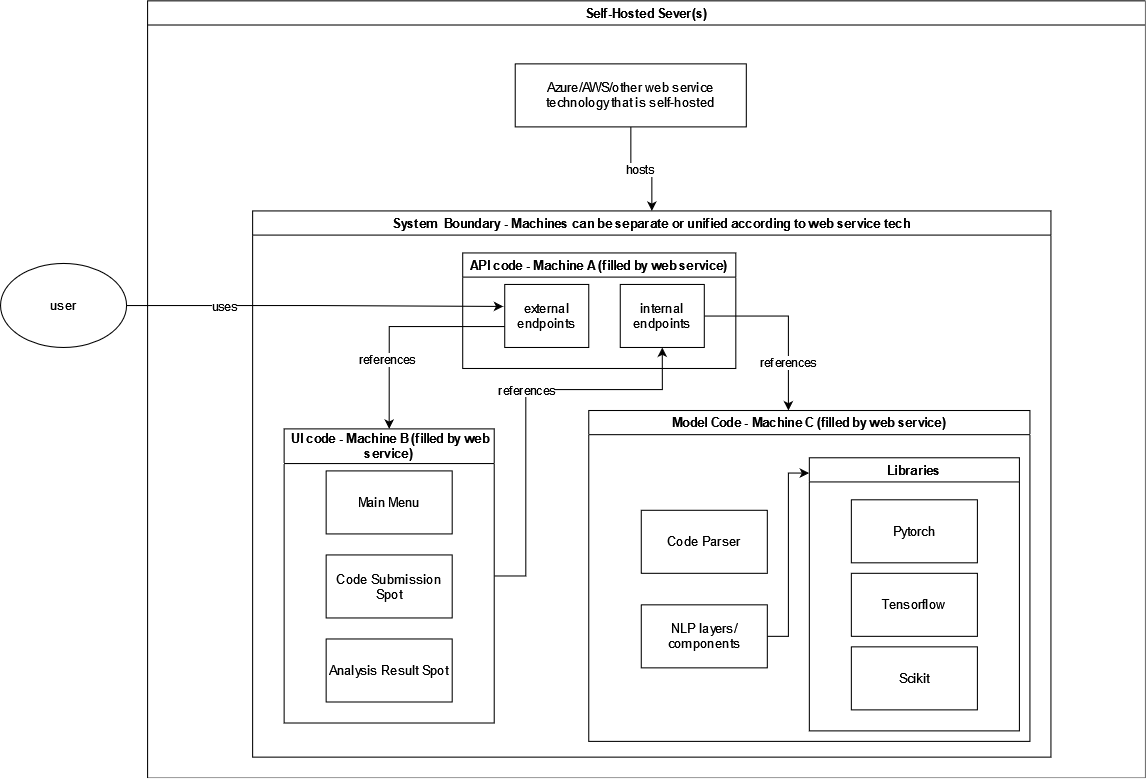
\includegraphics[height=.58\textheight]{./assets/Component_Border.png}
\caption{Diagram shows referential relationships, not workflows. System Boundary above surrounds all components our team will maintain and accept responsibility. A machine above is a server suitable to host code specified. Any machine mentioned above will not be provided to users from our project, they are expected to be self-hosted either on the user's own servers, or through technology such as Amazon Web Services (AWS) or Microsoft Azure.}
\end{figure}



\section{Critical Assumptions}
\begin{itemize}
    \item Adequate computational resources exist for the real time analysis of the code snippets
    \item Users do not intend to misuse the product
    \item Third party resources that support this product will always be functionally correct
    \item All components on the cloud will provide sufficient scalability and security
    \item The system will be maintained regularly with bug fixes/performance enhancements
    \item The criteria for plagiarism is agreed upon by all users
\end{itemize}

\section{Failure Mode and Effect Analysis}

\begin{landscape}
    \begin{table}[ht]
        \centering
        \caption{Failure Mode and Effect Analysis}
        \scalebox{0.7}{ 
        \begin{tabular}{|p{1.75cm}|p{4cm}|p{5cm}|p{5cm}|p{3cm}|p{5cm}|p{2cm}|p{2cm}|}
        \hline
        \textbf{Design Function} & \textbf{Failure Modes} & \textbf{Effects of Failure} & \textbf{Causes of Failure} & \textbf{Detection} & \textbf{Recommended Actions} & \textbf{SR} & \textbf{Ref.} \\
        \hline
        Input Processing & Failure to tokenize text & Model fails to function or gives wrong output & a. Code not in Python \newline b. Tokenizer malfunction \newline c. Corrupted file & Check file extension to ensure .py suffix & a. Check input beforehand \newline b. Notify user of error occurred & & H1-1 \\
        \cline{2-8}
        & Failure to upload file & Plagiarism detection process does not start & a. Invalid file type \newline b. Server error & Error handling & a. Notify user of failed upload & & H1-2\\
        \cline{2-8}
        \hline
        User Account Handling & Unauthorized access to account & a. Account compromised \newline b. User submissions compromised & a. Weak user authentication measures &  & a. Limit unsuccessful login attempts \newline  b. Multi-factor authentication & SR-A1 & H2-1 \\
        \cline{2-8}
        \hline
        Result processing and generation & Model is overfitted & Model fails to identify plagiarism for many inputs & a. Small dataset \newline b. Dataset too specific  & Test model with test dataset & a. Ensure datasets don't all have similar code & & H3-1\\
        \cline{2-8}
        & Model providing false positives & Submissions incorrectly flagged for plagiarism & a. Inability to recognize common coding practices \newline b. Error in model & Proper tests with test data split & a. Implement good pattern analysis \newline b. Proper testing & & H3-2\\
        \cline{2-8}
        & Comments are tokenized or ignored incorrectly & Comments become extremely easy way to bypass plagiarism detection & a. Bad implementation of model \newline b. Error in code & Found in testing using inputs with comments & a. Ensure code handles comments properly & & H3-3\\
        \hline
        Result output display & Results e-mail failed to send & Users who close the tab will not see the results & a. Network issues on either sender/recipient side \ newline b. Blocked by spam filters \newline c. Incorrect e-mail address & & a. Send e-mail from safe and trusted domains b. Ensure recipient address is filled correctly in script & & H4-1 \\
        \hline
        \end{tabular}
        } % End of \scalebox
        \label{table:fmea}
    \end{table}
\end{landscape}
   

\section{Safety and Security Requirements}

\begin{itemize}
\item \label{req:saf1} \textbf{SR-SAF1: Submission Rate Limitation}: The system shall limit the number of submissions by a parcitular user each day to prevent server overload.

Rationale: The activity of any user should not impact the performance of the system nor increase waiting times for other users.

\item \label{req:saf2} \textbf{SR-SAF2: Safe System States During Failure}: In case of system error (i.e. hardware or network failures), the system shall inform users of the failure of their pending submissions before gracefully shutting down.

Rationale: This ensures that users are notified of submission failures, preventing confusion or wasted time.

\item \label{req:saf3} \textbf{SR-SAF3: Warning of Potentially Inaccurate Detections}: In cases where the system produces detections with low confidence, the user shall be warned that the results may be inaccurate.

Rationale: Maintaining transparency that results may not be reliable protects users from acting on incorrect information before checking the results for themselves.

\item \label{req:saf4} \textbf{SR-SAF4: Protection Against Inappropriate Inputs}: The system shall validate all user submissions and reject malformed code submissions.

Rationale: Malformed inputs could lead to system crashes, incorrect analysis, or compromise system performance.

\item \label{req:saf5} \textbf{SR-SAF5: Isolation of Critical Functions}: Critical functions such as plagiarism detection and report generation shall be isolated from non-critical functionality to prevent faults in such non-critical components from affecting system stability.

Rationale: Issues in non-critical functions (such as the user interface) shouldn't compromise overall system stability.

\end{itemize}

\section{Roadmap}

This section outlines the implementation timeline for the safety and security requirements of the project. The following safety requirements will be prioritized and implemented as part of the capstone timeline, while others may be deferred for future releases to ensure complete and secure functionality. Note: Items appear in order of what will be implemented first.
\\ \\ \\
\subsection{Capstone Timeline Implementation}

\begin{itemize}
    \item \textbf{\hyperref[req:saf1]{SR-SAF1: Submission Rate Limitation}}
    \begin{itemize}
        \item \textbf{Description}: The system shall limit the number of submissions by a particular user each day to prevent server overload.
        \item \textbf{Rationale}: To ensure the system maintains optimal performance and prevents any user from monopolizing system resources.
        \item \textbf{Implementation Plan}: This will be implemented early on to mitigate any risks of server performance issues.
    \end{itemize}

    \item \textbf{\hyperref[req:saf2]{SR-SAF2: Safe System States During Failure}}
    \begin{itemize}
        \item \textbf{Description}: The system shall inform users of submission failures due to hardware or network errors and gracefully shut down.
        \item \textbf{Rationale}: Ensuring users are informed of system failures protects them from being left in the dark regarding their submissions.
        \item \textbf{Implementation Plan}: This feature will be crucial to handle system stability and to improve user experience, making it a priority during development.
    \end{itemize}

    \item \textbf{\hyperref[req:saf4]{SR-SAF4: Protection Against Inappropriate Inputs}}
    \begin{itemize}
        \item \textbf{Description}: The system shall validate all user submissions and reject malformed code submissions.
        \item \textbf{Rationale}: Prevents system crashes, incorrect analysis, or compromised performance due to malformed inputs.
        \item \textbf{Implementation Plan}: Will be integrated during the core system development phase to safeguard against harmful inputs.
    \end{itemize}

    \item \textbf{\hyperref[req:saf5]{SR-SAF5: Isolation of Critical Functions}}
    \begin{itemize}
        \item \textbf{Description}: Critical functions (plagiarism detection, report generation) shall be isolated from non-critical functions (UI) to prevent faults from spreading.
        \item \textbf{Rationale}: Ensures that non-essential issues do not impact the core stability of the system.
        \item \textbf{Implementation Plan}: This is critical for maintaining the integrity of the plagiarism detection system and will be developed alongside the primary features.
    \end{itemize}
\end{itemize}

\subsection{Future Releases}

\begin{itemize}
    \item \textbf{\hyperref[req:saf3]{SR-SAF3: Warning of Potentially Inaccurate Detections}}
    \begin{itemize}
        \item \textbf{Description}: The system shall warn users if detections have low confidence levels and could be inaccurate.
        \item \textbf{Rationale}: To maintain transparency with users, ensuring they do not rely on potentially incorrect results without further verification.
        \item \textbf{Future Implementation Plan}: This feature will be added after the initial release, once the confidence scoring mechanism has been thoroughly tested and refined.
    \end{itemize}
\end{itemize}

This roadmap ensures that the essential safety requirements are delivered as part of the capstone project, with further refinements and advanced features to be implemented in future iterations.

\newpage{}

\section*{Appendix --- Reflection}

\wss{Not required for CAS 741}

The purpose of reflection questions is to give you a chance to assess your own
learning and that of your group as a whole, and to find ways to improve in the
future. Reflection is an important part of the learning process.  Reflection is
also an essential component of a successful software development process.  

Reflections are most interesting and useful when they're honest, even if the
stories they tell are imperfect. You will be marked based on your depth of
thought and analysis, and not based on the content of the reflections
themselves. Thus, for full marks we encourage you to answer openly and honestly
and to avoid simply writing ``what you think the evaluator wants to hear.''

Please answer the following questions.  Some questions can be answered on the
team level, but where appropriate, each team member should write their own
response:


\begin{enumerate}
    \item What went well while writing this deliverable?

    Ascertaining what our system boundary was went particularly well. It had 
    us more formally identify what components exist for development along 
    with where hazards could occur within said components. This more rigorous
    process of determining system components had our team unify further on
    how we can potentially implement aspects of our product, giving a clearer
    vision for the future development path. More importantly, the rest of the 
    deliverable became much smoother once we could isolate components
    for hazards instead of attempting to inspect the entirety of our project 
    at once.

    \item What pain points did you experience during this deliverable, and how
    did you resolve them?

    It was unclear at first what actions had to be taken to reconcile 
    requirements made or referenced in this document with our SRS. For example, 
    we were not certain about referencing our SRS requirements through some 
    form of hyperlink or if requirements added in the hazard analysis document 
    needed an entirely new section in the SRS. We resolved this by clarifying 
    with the TA during our meeting for this deliverable. We were also unsure 
    about the timeline of implementation of our requirements to address 
    identified hazards. It was not certain what would be realistic. We 
    addressed this using our intuition by giving what we thought were fair 
    priorities to each hazard, and ordering the addressal of hazards based on 
    these priorities. We also kept the timings a bit more vague to give us 
    breathing room incase something changes.

    \item Which of your listed risks had your team thought of before this
    deliverable, and which did you think of while doing this deliverable? For
    the latter ones (ones you thought of while doing the Hazard Analysis), how
    did they come about?
    
    Old ones: model providing false positives, failure to upload file, 
    model is overfitted, Unauthorized access to account

    New ones: results in email failed to send, failure to tokenize text, 
    Comments are tokenized or ignored incorrectly

    The new ones came about mainly thanks to the components identified in the 
    system boundary. Before, we did not isolate the parser in its functionality 
    from the model itself nor did we think about adversarial ways to trick the 
    parser, such as comments. We also did not consider the output failing to 
    reach the user via email. This was identified thanks to an exercise where we 
    outlinted all ways output could reach a user and found we originally just
    considered on-screen failures, and not failures external to our UI display.
    

    \item Other than the risk of physical harm (some projects may not have any
    appreciable risks of this form), list at least 2 other types of risk in
    software products. Why are they important to consider?

    Security Risks - Even if a user is not physically harmed directly by software,
    it is important a software does not set them up for other forms of harm such
    as mental, financial, or reputational, by revealing their identity, location, or
    any specifics about them that they do not wish to be publicly known. Any of 
    such pieces of information could potentially be used to blackmail the user 
    and endanger them. This type of risk is relevant in our product too, seeing 
    it deals with sensitive user data, like user code submissions and generated 
    plagiarism detection reports. Safeguarding that information prevents people 
    from having their coding ideas stolen and their reputations from being 
    damaged with possible accusations of plagiarism.

    Performance Risks - One of the priorities of a product besides doing no 
    harm is in fact to do good, or rather, to fulfill a function. If a product 
    is not able to run and conduct tasks for the user consistently, it can 
    annoy a user if not downright harm them depending on the criticality of the 
    product's task. Therefore, it is important that a product maintains 
    consistent computational abilities to uphold expectations of the user when
    it comes to producing results at a certain rate. This type of risk is also
    one we have had to consider for our product since it requires a lot of 
    computational power to function. Not providing sufficient support in terms of
    gpus for our model can have it fail to give an output in an adequate time
    period, meaning users would stop using our product altogether. Given that we 
    plan to support multiple users concurrently, it is very important we mind the 
    resources necessary to keep our product fast and responsive. An unusable 
    product is akin to no product.


\end{enumerate}

\end{document}